%% 2016/07/25
%% by Sylvain Chatel
%% See:
%% sylvain.chatel@supelec.fr
%% Report paper on the cyber security of the distributed model predictive control

%% This work is distributed under a CC-BY License.
%%*************************************************************************

\documentclass[conference, peerreview]{IEEEtran}
\usepackage[utf8]{inputenc}
\usepackage[T1]{fontenc}
\usepackage[francais]{babel}
\usepackage{graphicx}
\usepackage{mathrsfs}
\usepackage{color}
\usepackage{colortbl}
\usepackage{amsfonts}
\usepackage{amssymb}
\usepackage{graphicx}
\usepackage[top=2cm, bottom=2cm, left=2cm, right=2cm]{geometry}
\usepackage{mathrsfs}
\usepackage{textcomp}
\usepackage{nccmath}
\usepackage{pgf}
\usepackage{float}
\usepackage{schemabloc}
\graphicspath{{graphique/}}
\usepackage{stmaryrd}
\usepackage{bm}

% *** CITATION PACKAGES ***
%
\usepackage{cite}

% *** MATH PACKAGES ***
%
\usepackage{amsmath}

% *** ALIGNMENT PACKAGES ***
%
\usepackage{array}

% correct bad hyphenation here
\hyphenation{op-tical net-works semi-conduc-tor}
\edef\hc{\string:}

\begin{document}
%
\title{Security of the Distributed Model Predictive Control }


% author names and affiliations
% use a multiple column layout for up to three different
% affiliations
\author{\IEEEauthorblockN{Sylvain Chatel, Pierre Haessig and Romain Bourdais.}
\IEEEauthorblockA{CentraleSupélec - IETR - UMR 6164, France\\
Email: sylvain.chatel@supelec.fr, $\{$pierre.haessig ; romain.bourdais$\}$@centralesupelec.fr
}
}

% make the title area
\maketitle
\thispagestyle{plain}
\pagestyle{plain}


\begin{abstract}
In this paper, we explored the security of a distributed model predictive control (DMPC) scheme. A global system is decomposed into several local subsystems. Each subsystem owns a model predictive control (MPC) controller which cooperates and works iteratively with all the other controllers in order to reach the system's objective. Here, we focus on the security of such a system. Indeed, we noticed that a user could disturb the DMPC through several attacks in order to destabilize the resource distribution. Hence, examples of cheating protocols and counter-cheat ideas were discovered and are presented here. 
\end{abstract}

% For peer review papers, you can put extra information on the cover
% page as needed:
\ifCLASSOPTIONpeerreview
\begin{center} \bfseries EDICS Category: \textsc{ Peer Review  : v 1.0} \end{center}
\fi
%
% For peerreview papers, this IEEEtran command inserts a page break and
% creates the second title. It will be ignored for other modes.
\IEEEpeerreviewmaketitle



\section{Introduction}
Model predictive control (MPC), also known as \textit{receding horizon control}, is becoming more and more popular in the industrial process control \cite{Venkat, Campo}. Among other perks, the attractiveness of the MPC lies in its ability to represent clearly the constraints of the optimization problem \cite{Jia}. Over the past decades, the MPC has become widespread and many successful applications have been developed in the process industry. 

In an MPC, the objective is to get the optimal control input over a given horizon by solving a discrete-time optimal control problem. Traditionally, this kind of control is done by a controller in a centralized way.  This controller have full knowledge of the system over the horizon. Although efficient, this schemes might sometimes be inadequate. For instance,  for large-scale interconnected systems such as power and water distribution or even traffic systems (with plug and play), a centralized MPC might not be ideal or even technically feasible \cite{Jia}. Moreover, the fact that the controller is omniscient and  fully knowledgeable might be an obstacle because some agents might not be able to divulge information about their local subsystem. This might be the case as \cite{Campo} points out for the newly regulated power markets in the United States.

Hence the idea of developing a distributed system. The global system is decomposed into several subsystems. Each subsystem has a MPC controller which communicates with the others. Local control inputs are then locally computed and determined with the few information shared. For instance, when a decentralized control scheme (where local control input are determined based on local measurements for instance) is needed, a distributed MPC is a better choice. For example, for water distribution systems, a centralized MPC is decomposed into a DMPC using a coordinator (e.g. augmented Lagrangian \cite{Campo} or Uzawa method \cite{Cohen}).

Several distributed MPC examples are available in the literature. DMPC frameworks were developed in \cite{Acar, Sawa} and \cite{ Dunbar}. In the latest, a MPC framework is developed for a system with several independent subsystem dynamics but nonetheless linked through their cost functions. 

In a DMPC, each agent communicates with the others via a simple coordinator. This latest, returns a simple information (e.g. a Lagrangian multiplier for an augmented Lagrangian technique). All the information required for the system to work efficiently is communicated through this small amount of data. As pointed out  in \cite{Brooks}, though efficient the DMPC still suffers from some risks. Indeed, DMPC might sometimes be harmful to the physical system. For instance in a complex system, human error, malicious and misleading agents could easily disturb the grid. According to Brooks in \cite{Brooks}, one of the best ways to mitigate those security threats is to involve a combination of counter measures such as using fault detection softwares, limiting the size of each entity or even certifying aggregators. However, to the best of our knowledge for the first time security threats and counter measures were comprehensively studied. 

The paper is organised as follow.  Section II introduces the model of DMPC for power distribution  we used in our study. In Section III,  a study of the base cases is conducted. The security threats are implemented and studied in section IV. In Section V, the main contribution of this study are summarized. 


\section{Model}
In this paper, we consider a linear time-invariant (LTI) system composed of $m$ interconnected subsystems. Each subsystem represent a room with a thermal resistance $R_{th}$ and a thermal conductivity $C_{th}$. Taking into account the exterior temperature $T_{ext}$, the objective is for the temperature of each room $T_i$ to be as close as possible to the reference temperature $T_{id}^i$ at each time. All rooms are getting their energy from a limited global amount of energy $U_{max}$, and each user has a maximum  admissible energy $u_{max}^i$ due to its physical configuration. We note $u_i$ the energy consumed by user i. Since the consumed energy cannot exceed the maximum admissible energy, and since the global energy resource is limited, we have the first two constraints :

\begin{equation}
\forall i \in \llbracket 0, m-1 \rrbracket, \; 0 \leq  u_i \leq  u_{max}^i 
\label{uimax}
\end{equation}

\begin{equation}
\sum_{i = 0}^{m-1} u_i \leq U_{max}
\label{umax}
\end{equation}

In order to take into account the will of each user to reach its ideal temperature, we introduced a comfort factor $\alpha$.  Hence the optimization problem is to minimize the following cost function subjected to \ref{uimax} and \ref{umax}. 

\begin{equation}
J_u = \sum_{i = 0}^{m-1} u_i  \; + \; \sum_{i = 0}^{m-1} \alpha_i (T_i - T_{id}^i)^2 
\label{cost}
\end{equation}

In order to determine the $J_u$, we used the thermal model presented in Figure \ref{thermmod}.

\begin{figure}[!t]
\centering
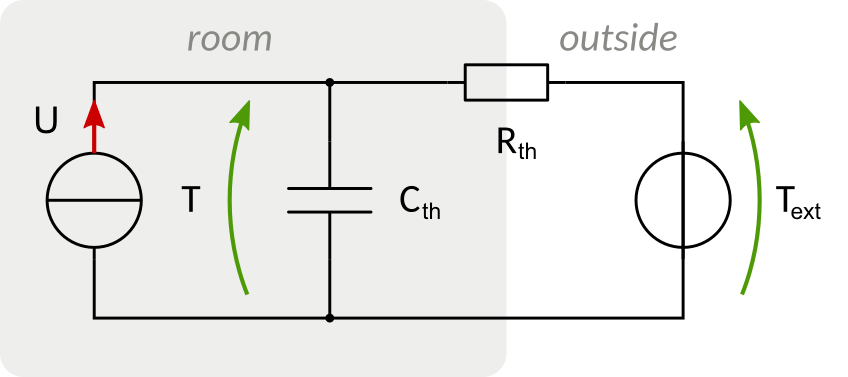
\includegraphics[width=3in]{therm_diagram.png}
\caption{Thermal model of a room. $R_{th}$ represents the thermal resistance and $C_{th}$ the thermal conductivity of the room. $U$ is the consumed power, $T$ the temperature of the room and $T_{ext}$ the external temperature.}
\label{thermmod}
\end{figure}

With this model, it is possible to use the state-space representation of the problem. We can  set $\bm{X}[k]$ as the temperature vector of each room. $\bm{U}[k]$ represents the consumed energy of each room and $\bm{U}_{ext}[k]$ the external temperature. 
With those notations, we can write:

\begin{equation}
\bm{X}[k+1]\; = \; A . \bm{X}[k] + B .\bm{U}[k] + B'.\bm{U}_{ext}[k]
\label{state}
\end{equation}

Given equation \ref{state}, and the model, we can replace the temperature in equation \ref{cost}. This enables us to have a quadratic problem in $\bm{U}$ :

\begin{equation}
J_u = \bm{U}^T P \bm{U} + q^T \bm{U} + cst 
\label{cost_en}
\end{equation}

In order to proceed to a centralized MPC, we just have to minimize \ref{cost_en} subjected to \ref{uimax} and \ref{umax}. However, in order to have a DMPC, we need to decompose the computation to all users. To this end, we used an Uzawa method. The idea is to unconstrain  the optimization problem and relax the constraint in \ref{umax}. Then, after solving the optimization problem, we iterate the Lagrangian multiplier $\lambda$.
\begin{equation}
\lambda_{k+1} = \lambda_k + p * (\sum_{i=0}^m u_i^*[k] - U_{max})
\label{lambda}
\end{equation}
In \ref{lambda}, $p$ represents the step of the Uzawa iteration and $u_i^*[k]$ the optimal consumption of user i at k. This iterative procedure is done until the difference between $\sum_{i=0}^{m-1} u_i^*[k]$ and  $U_{max}$ is lower than a threshold. We note $\lambda_{opt}$ the value of the multiplier fulfilling this condition.

\begin{figure}[!t]
\centering
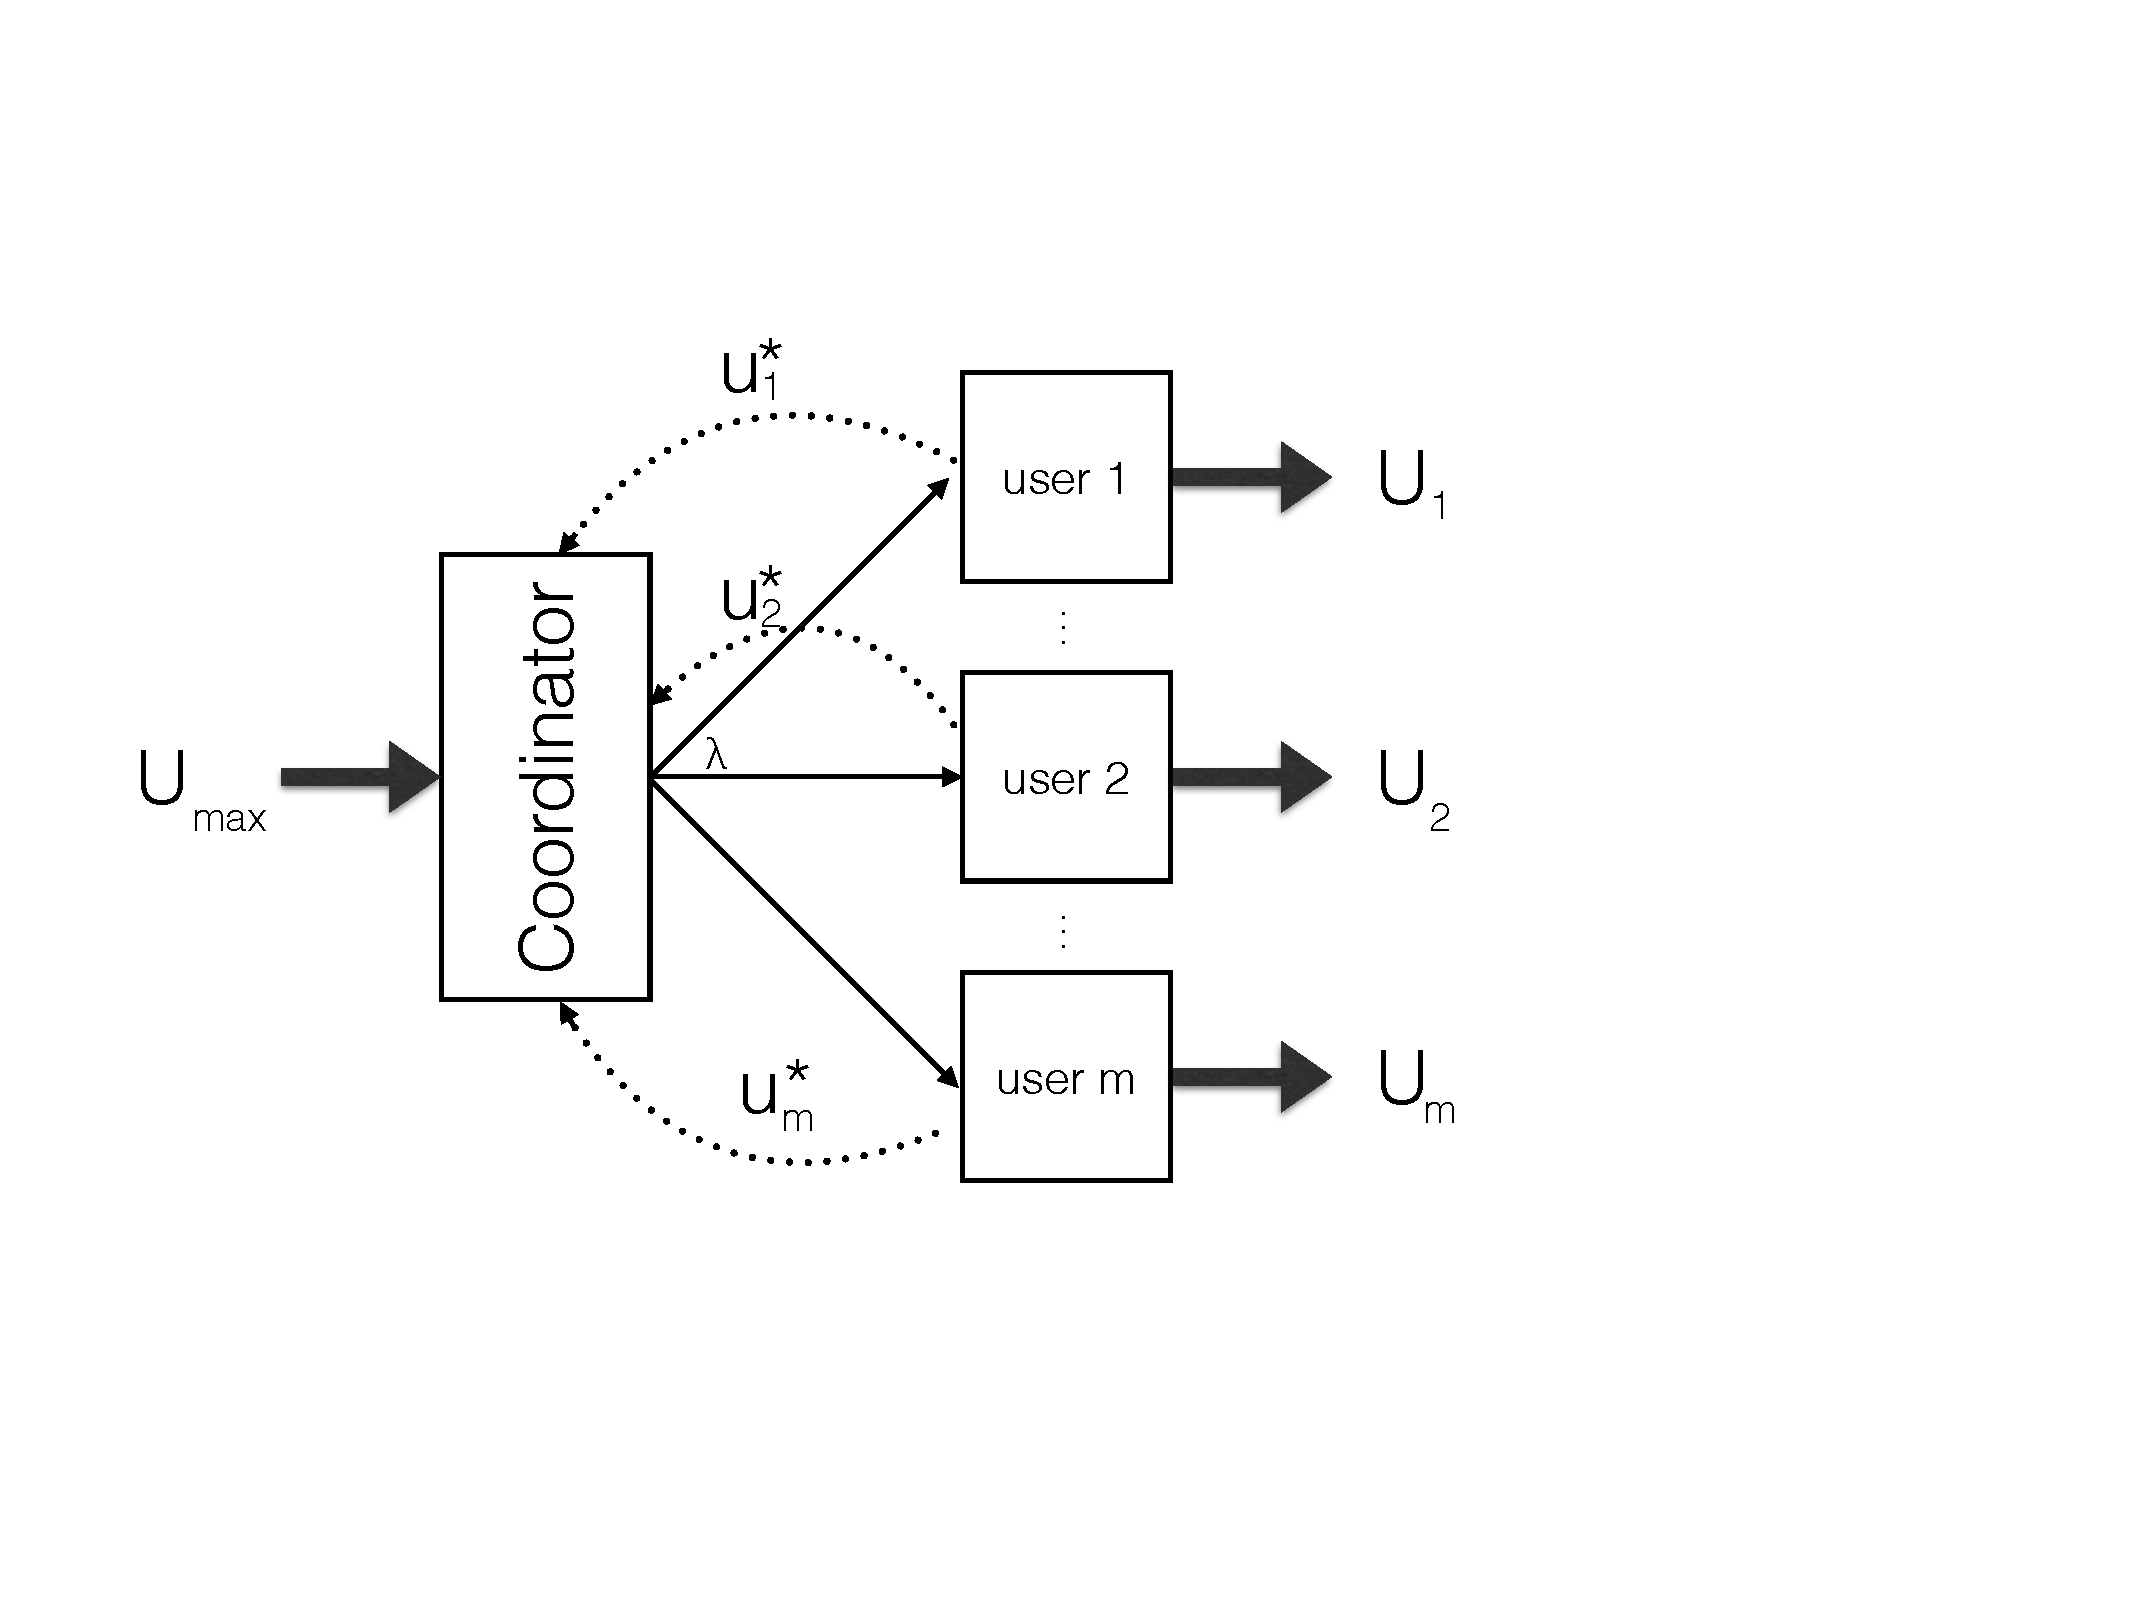
\includegraphics[width=3in]{ASHschema}
\caption{Structure of the distributed problem}
\label{coord}
\end{figure}
To summarize, the DMPC requires to solve the following quadratic problem over a prediction horizon $N$ for a simulation lasting over $N_{sim}$ :
\begin{equation}
\left\{
\begin{array}{l}
\text{min} \; J_u[j] =   \bm{U[j]}^T P \bm{U}[j] + q^T \bm{U}[j] + cst[j] + \lambda[k_{opt}]  \\
\text{subjected to}\\
\forall j  \in \llbracket 0, N_{sim}-1 \rrbracket, \forall i \in \llbracket 0, m -1 \rrbracket, \; 0 \leq  u_i \leq  u_{max}^i
\end{array}
\right.
\label{QP}
\end{equation}

In our case study, we opted for $N_{sim} = 24$ h.  

\section{Base cases}
In this section, we present the results for the nominal experiment of power distribution in several cases : the static case, the centralized dynamic case and the distributed dynamic case. All those simulations were made via the python module we developed. This package relies on M. Andersen and L. Vandenberghe \textit{cvxopt} package for convex optimization \cite{Boyd}.

\subsection{Static case}
\subsubsection{Centralized case}

Let us consider a problem with three different users. We consider, at first, that all users are identical. We set the system so that $U_{max}$ is inferior to the sum of all admissible temperature. 
\begin{figure}[H]
\centering
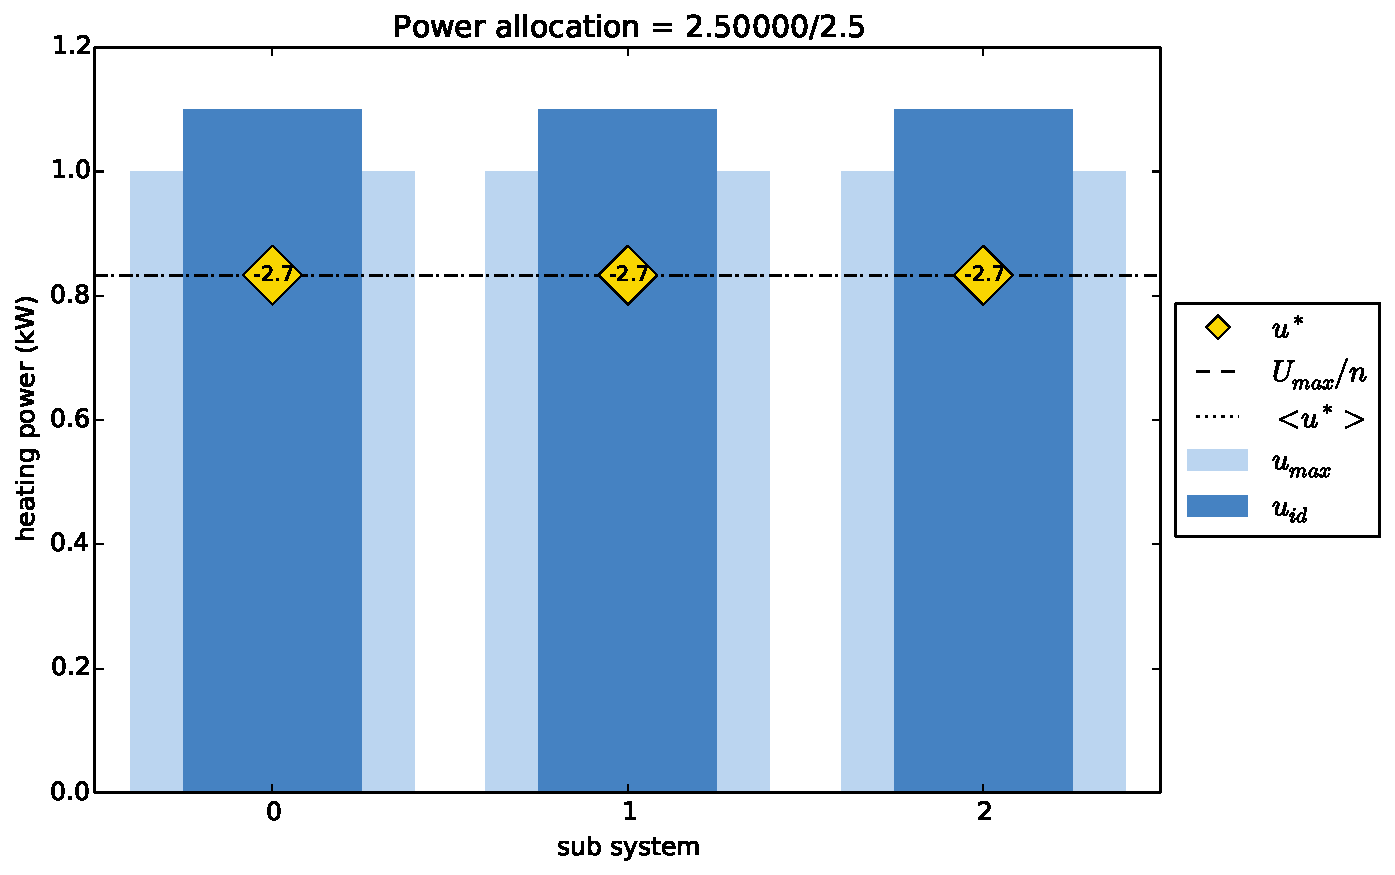
\includegraphics[width=3in]{static_PB_init.pdf}
\caption{Optimal power distribution in a static symmetrical case}
\label{statPBinit}
\end{figure}

Now, if we change the comfort factor of the third user in order for him to be more comfortable. To do so, let us take $\alpha_2 = 10\times  \alpha_0 $.

\begin{figure}[H]
\centering
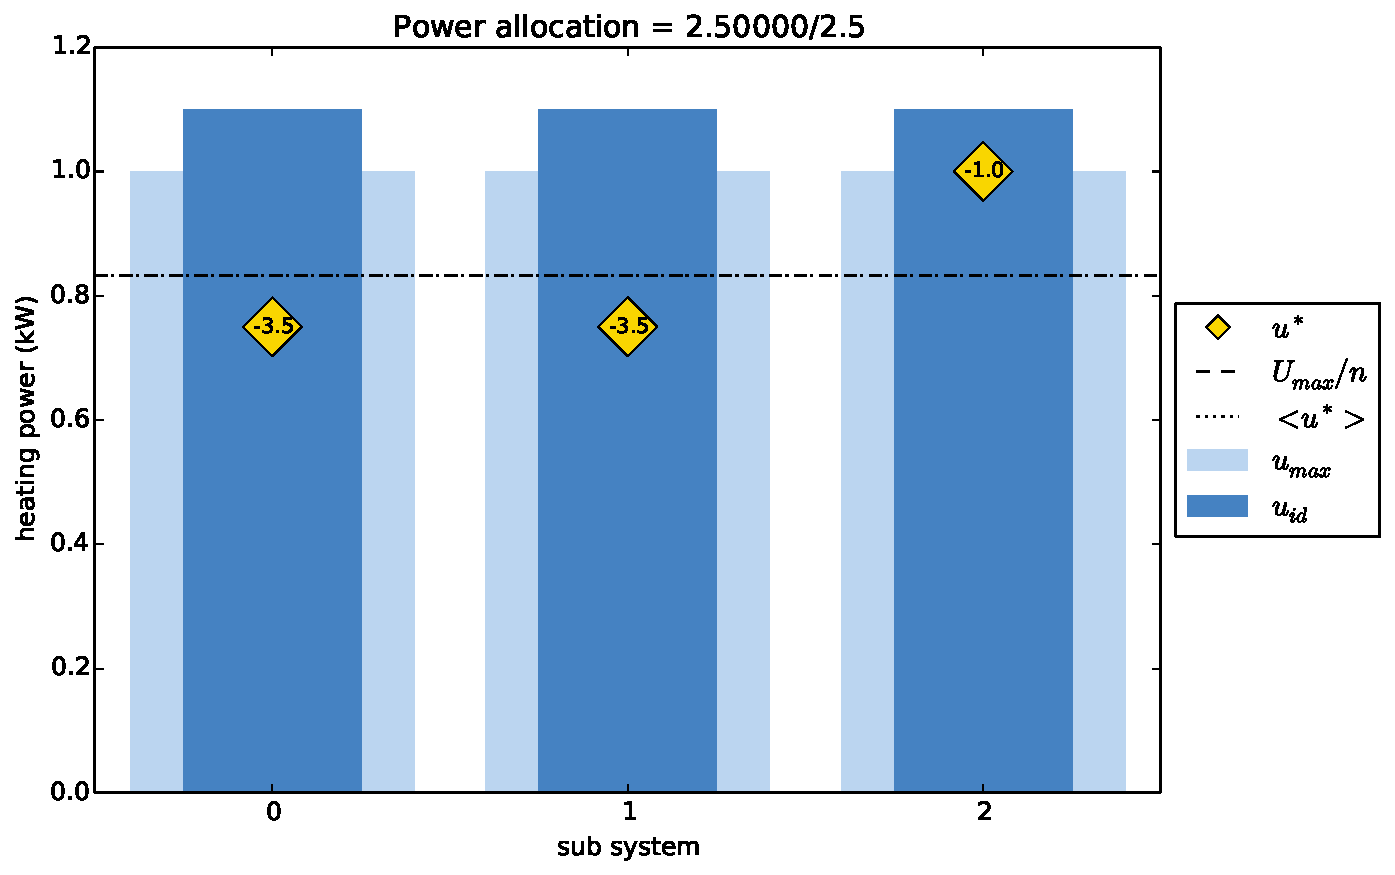
\includegraphics[width=3in]{static_PB_cht.pdf}
\caption{Optimal power distribution in a static case with different priorities, $\alpha_2 / \alpha_0 = 10$ }
\label{statPBcom}
\end{figure}

When comparing Figure \ref{statPBinit} and \ref{statPBcom}, we notice that the third user ($n^{\circ}2$ is indeed preferred in the power distribution and then its comfort becomes better to the disadvantage of the others (i.e. the square deviation to the ideal temperature of the third user ($n^{\circ}2$ is the smallest of all users).

\subsubsection{Distributed case}
When we decompose the centralized computation with the Uzawa method, we are able to model a distributed optimization. At first we consider a symmetrical situation.  
\begin{figure}[H]
\centering
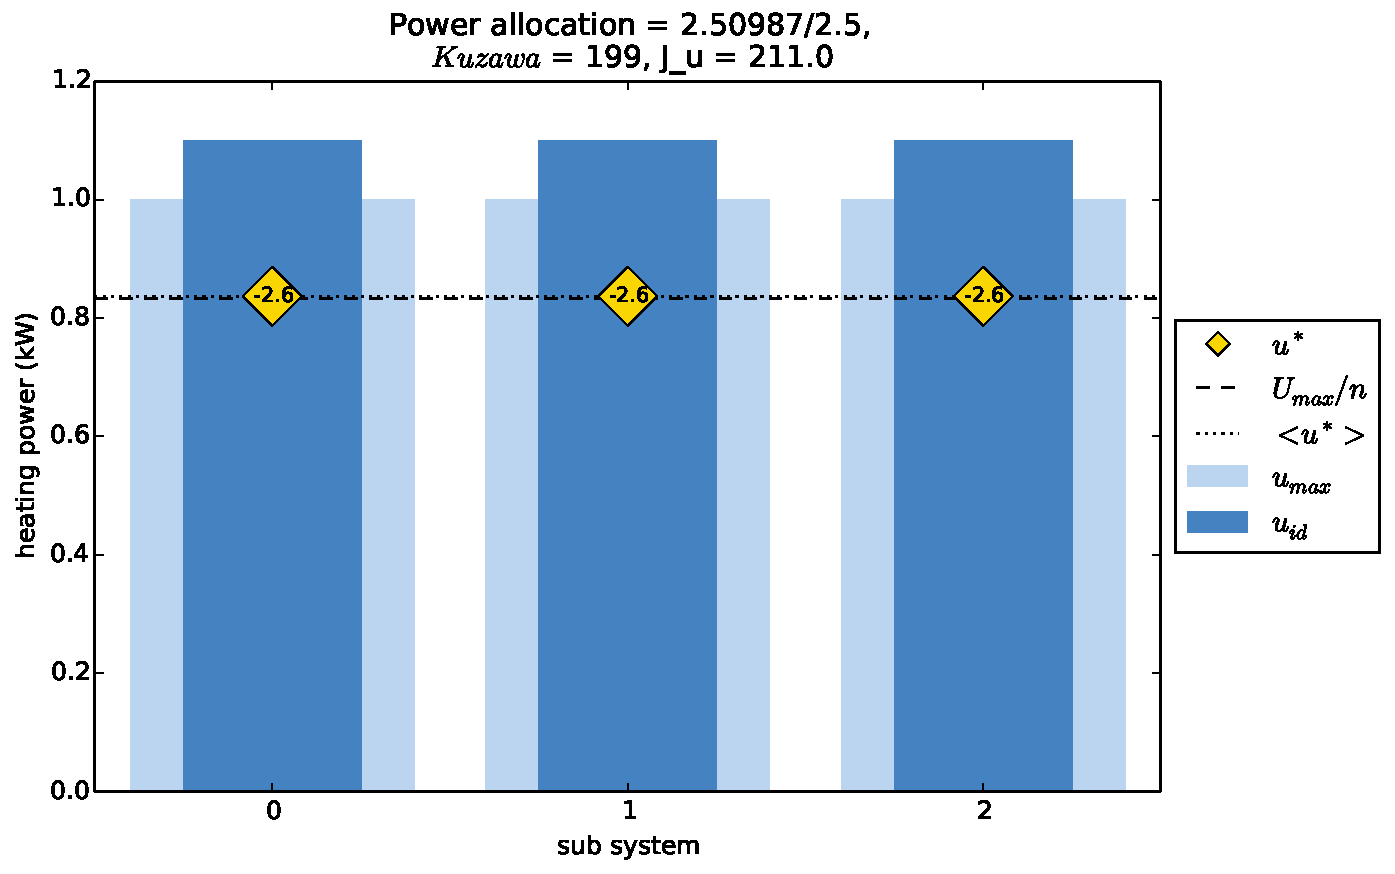
\includegraphics[width=3in]{static_DPB_init.pdf}
\caption{Optimal power distribution in a static symmetrical distributed case}
\label{statDPBinit}
\end{figure}

Now, if we change the comfort factor of the third user in order for him to more comfortable. To do so, let us take $\alpha_2 = 10 \times \alpha_0 $.

\begin{figure}[H]
\centering
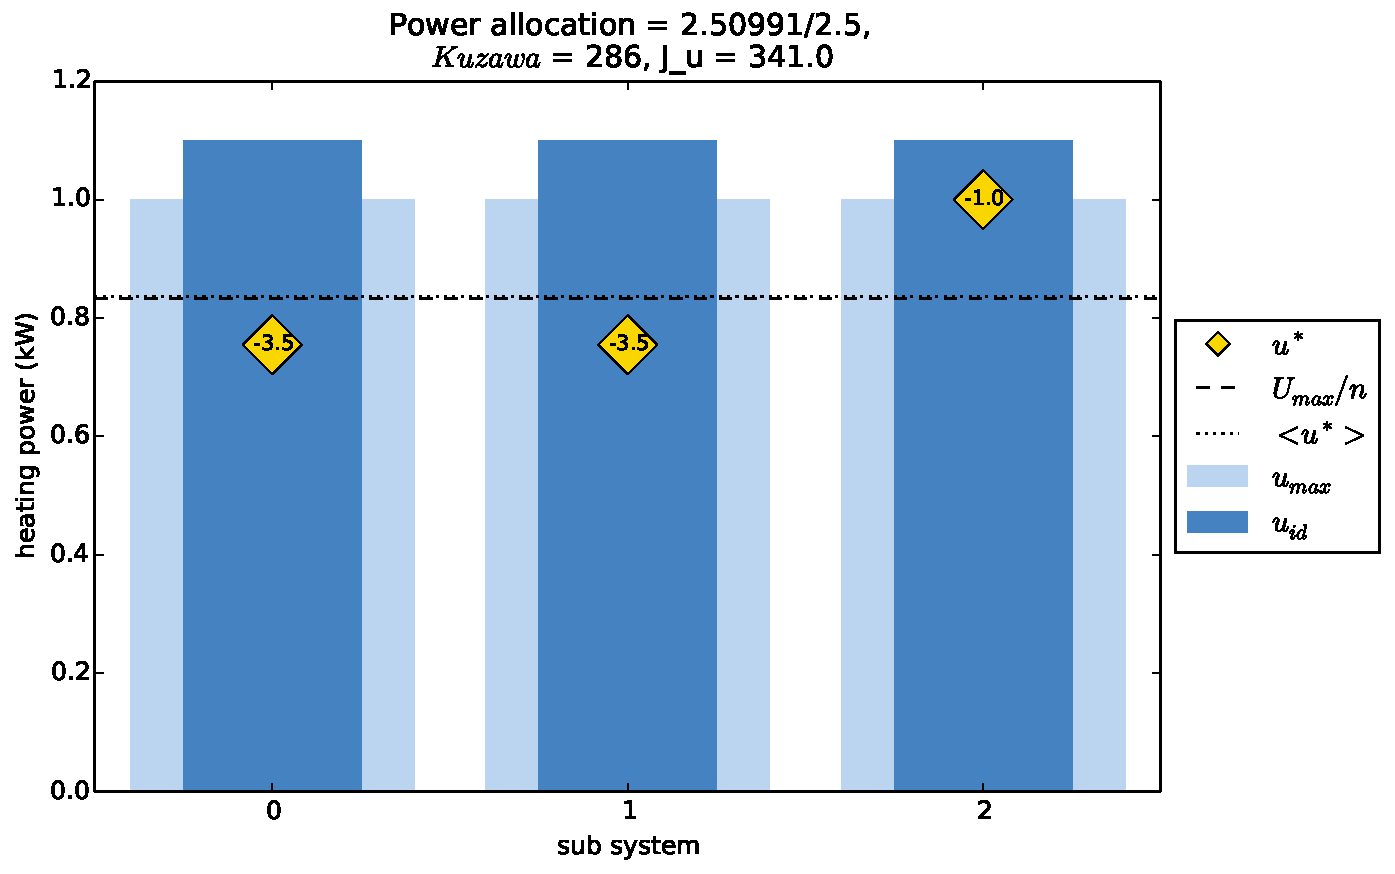
\includegraphics[width=3in]{static_DPB_cht.pdf}
\caption{Optimal power distribution in a static distributed case with different priorities, $\alpha_2 / \alpha_0 = 10$}
\label{statDPBcom}
\end{figure}
 
 When comparing Figure \ref{statDPBinit} and \ref{statDPBcom}, we notice as before that the third user ($n^{\circ}2$ is more satisfied to the disadvantage of user 1 and 2. We notice as well that the total amount of consumed energy is superior to $U_{max}$. This phenomenon is due to the constraint relaxation executed in the Uzawa method.
 
 Through this nominal static study, we were able to determine the influence of all the different parameters on the optimal solution among which the Uzawa step determination  in order to have a convergence of the Uzawa iteration.  We then used those results in the study and set $p = 1.5$.
 
 \subsection{Dynamic case}
 Now, we consider a dynamic simulation on a horizon of 24 hours. Three different users are using a limited amount of energy $U_{max}$. The ideal temperature is determined with a time based profile : between 6\hc 30-8\hc 30 am and 18\hc 00-22\hc 00 pm the user wishes to have a temperature $T_{pres}$ (people are present in the room), the rest of the time the temperature is set to $T_{abs}$. 
 
\begin{figure}[H]
\centering
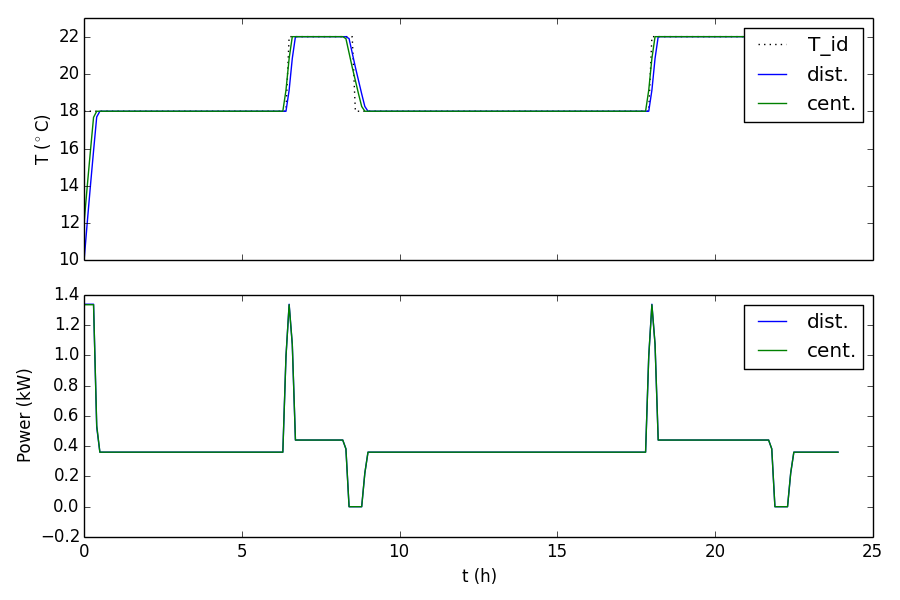
\includegraphics[width=3in]{dynDMPC_init.png}
\caption{Optimal power distribution in a dynamic case for user 2 in a symmetrical problem}
\label{dynDPBinit}
\end{figure}
\begin{figure}[H]
\centering
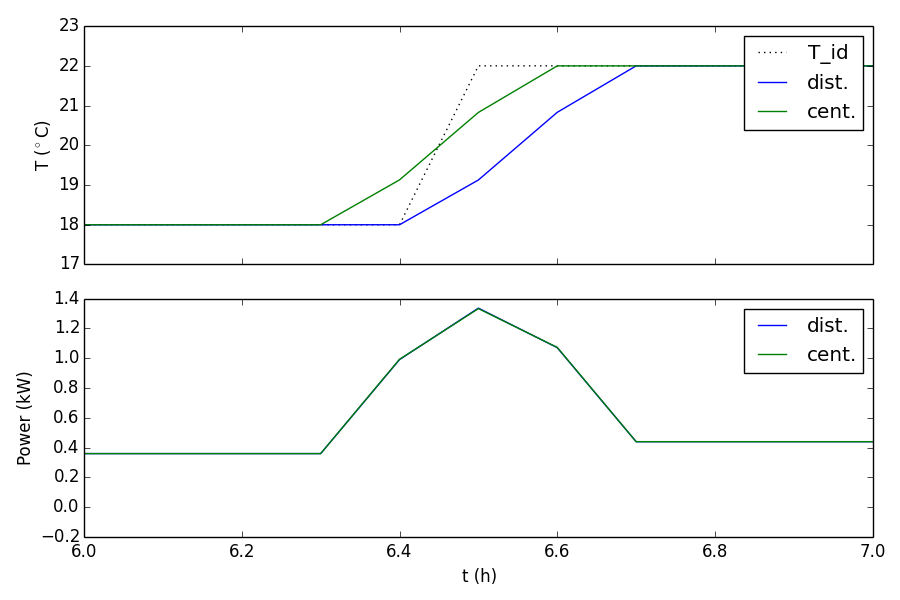
\includegraphics[width=3in]{dynDMPC_initZOOM.png}
\caption{Optimal power distribution in a dynamic case for user 2 in a symmetrical problem, focus between 6\hc 30-8\hc 30 am}
\label{dynDPBinit}
\end{figure}

As before, we now consider a situation where user 2 is preferred and has a comfort factor ten times superior to others. 
 
\begin{figure}[H]
\centering
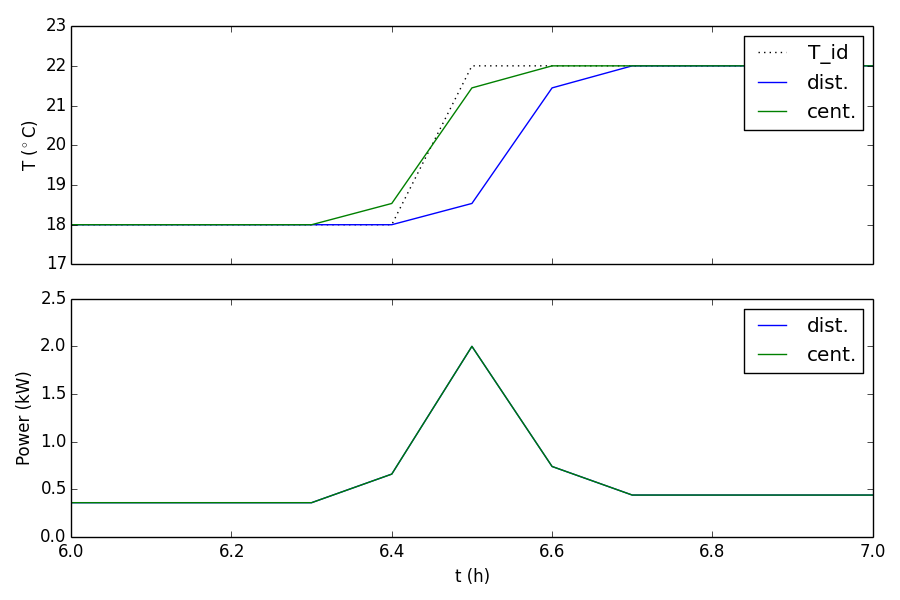
\includegraphics[width=3in]{dynDMPC_chtZOOM.png}
\caption{Optimal power distribution in a dynamic case for user 2 when it is preferred, $\alpha_2 / \alpha_0 = 10$, focus between 6\hc 30-8\hc 30 am }
\label{dynDPBcom}
\end{figure}
 We notice comparing Figures \ref{dynDPBinit} and \ref{dynDPBcom} that in the second case, user 2 is given mush more energy when needed and hence can reach its ideal temperature much faster.

From this point on, we are able to use this model to begin the study of cheating and misleading scenarios.
  
\section{Security issues : misleading and cheating users}
In this section, we will focus on the security issues of the DMPC. First, we will analyse the different ways of cheating before putting it into application on static and then dynamic situations. 

\subsection{Security concepts}
First of all, we must clarify the concept of security breach in a DMPC. Through our research, we were able to detect two kinds of threatening users : greedy users (whose objective is to maximize their comfort) and nihilist users (whose objective is to destroy the system). 

 \begin{figure*}[!t]
\centering
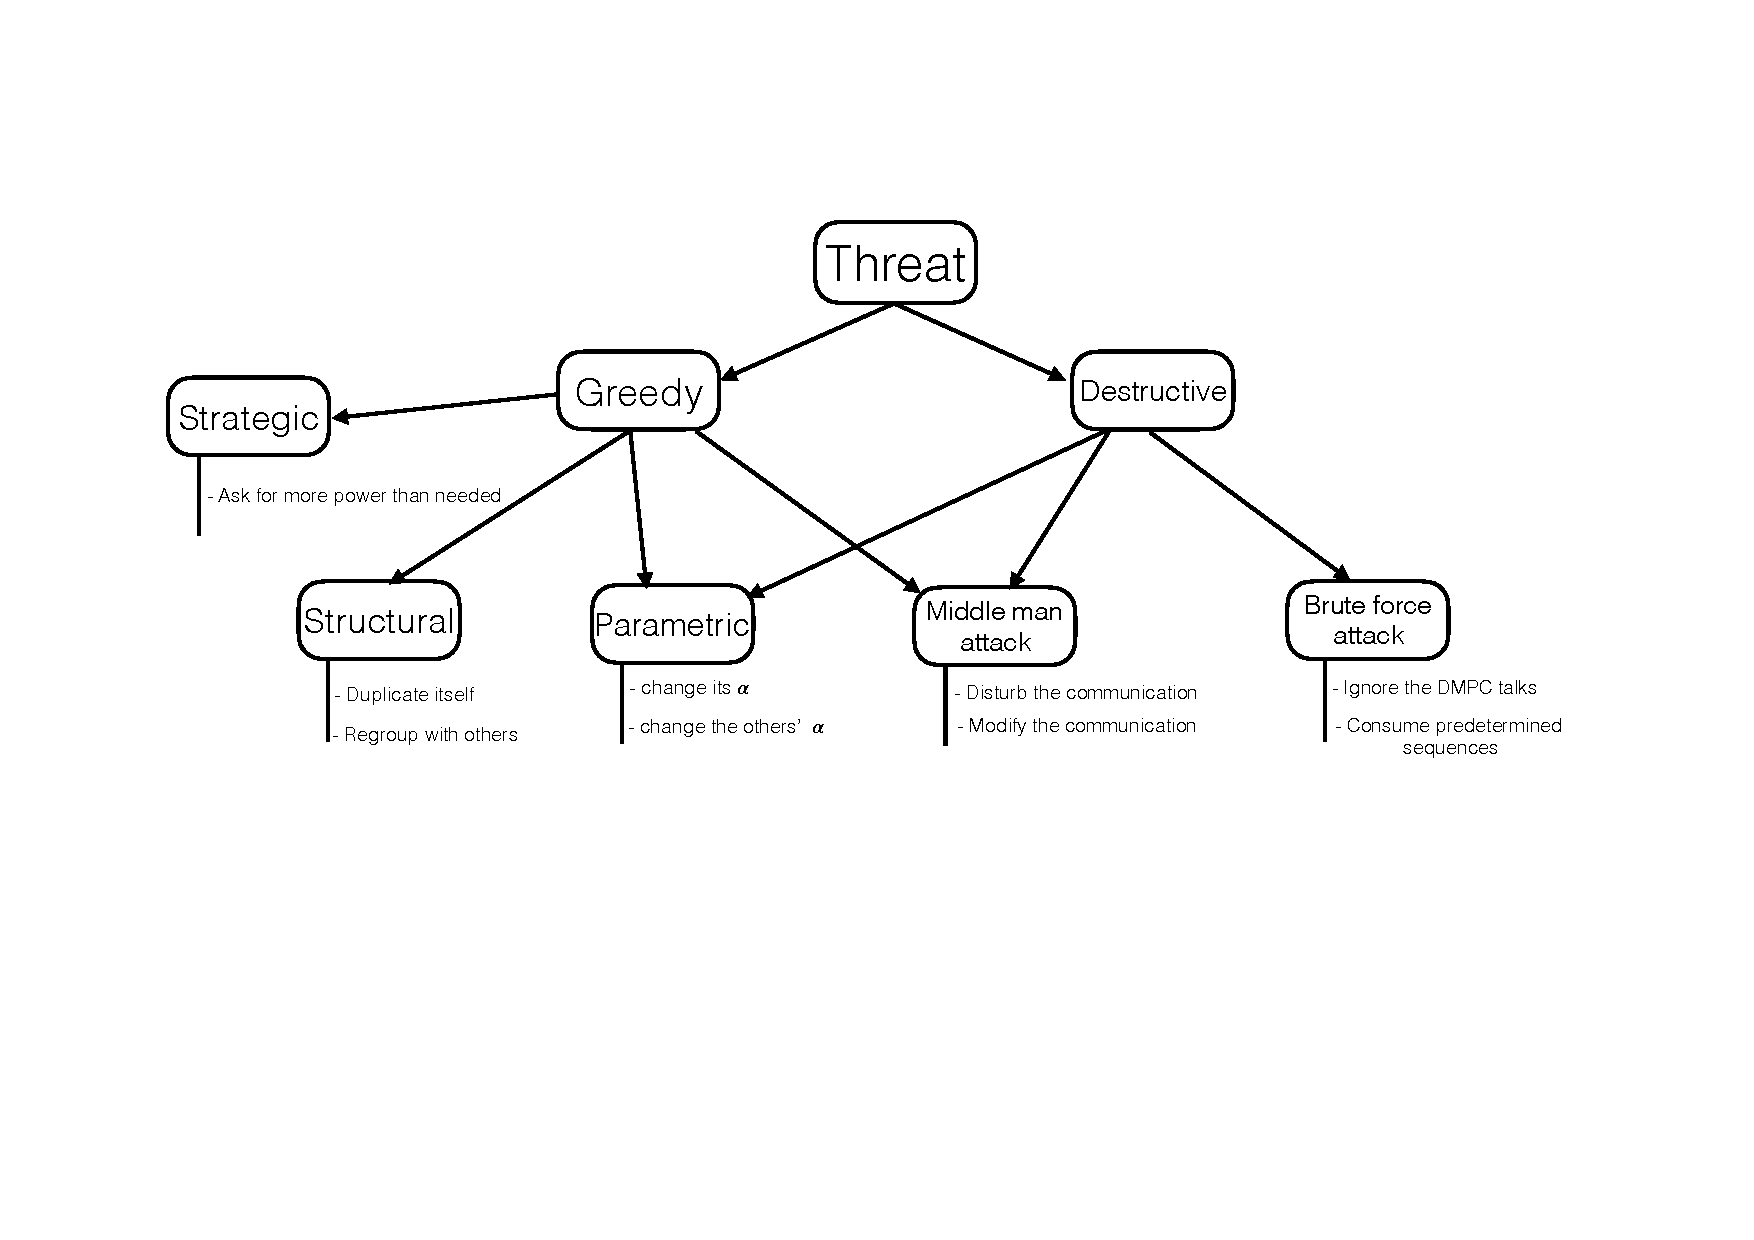
\includegraphics[width=5.5in]{mindmap}
\caption{Overview of different threatening methods}
\label{mindmap}
\end{figure*}

In Figure \ref{mindmap}, we can see an overview of the different threat we detected. The reader can note that even if other strategies might exist, we realized  that all the other strategies can be somehow reduced to one of those we studied. 

Moreover, for our study we considered that the transmission canal is ideal and that the communication cannot be altered. Indeed with the current knowledge, security protocols enable us to safely communicate and to change ones identity. This implies that in our model cheating by usurping ones identity or by altering the communication is not considered. Moreover, unless the demand profile of the users are complementary, the strategy of regrouping is ineffective. \\

To summarize, the base threatening cases are as follow : 
\begin{itemize}
\item[•] Change its own comfort factor $\alpha_i$.
\item[•] Change its broadcasted ideal temperature.
\item[•] Do not listen to the DMPC talks.
\item[•] Listen partially to the DMPC talks.
\item[•] Duplicate itself.
\end{itemize}

\subsection{Security in static situations}
Now, we implement those strategies into the static model. 

First, we implemented the influence of the comfort factor $\alpha$. The idea was to determine to which extent this parameters changes the power distribution. In Figure \ref{SCHT_a2}, we represented the optimal power distribution and the temperature deviation for two users when the comfort factor is a parameter. We noticed that, as expected, when the one user comfort factor is superior to the one of the others,  it receives much more energy and as therefore a better comfort. In Figure \ref{SCHT_a5}, we notice that the more users there are against a user who changes its comfort factor, the more they are neglected in regard to the cheater.

\begin{figure}[H]
\centering
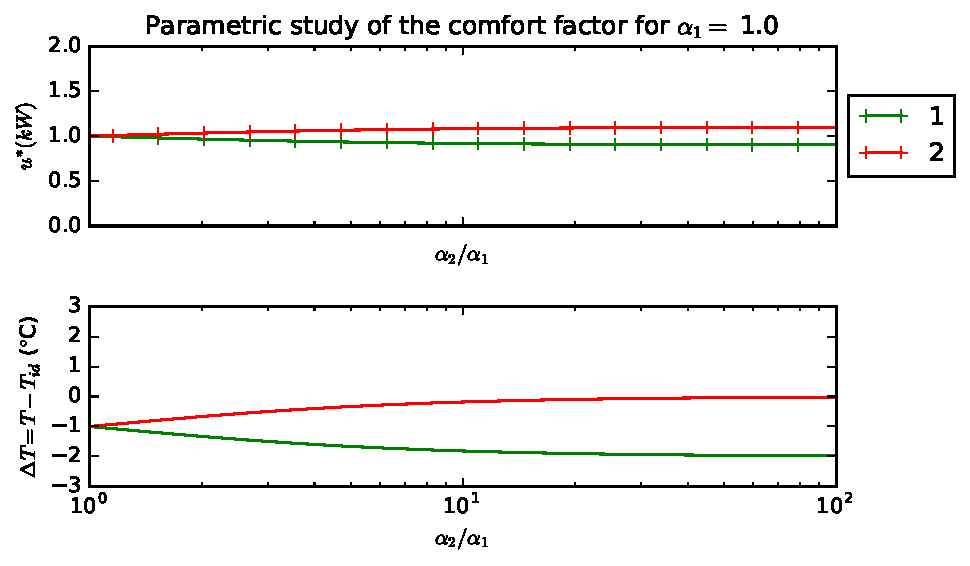
\includegraphics[width=3in]{statcht2alpZ.pdf}
\caption{Parametric study of the comfort factor for two users}
\label{SCHT_a2}
\end{figure}

\begin{figure}[H]
\centering
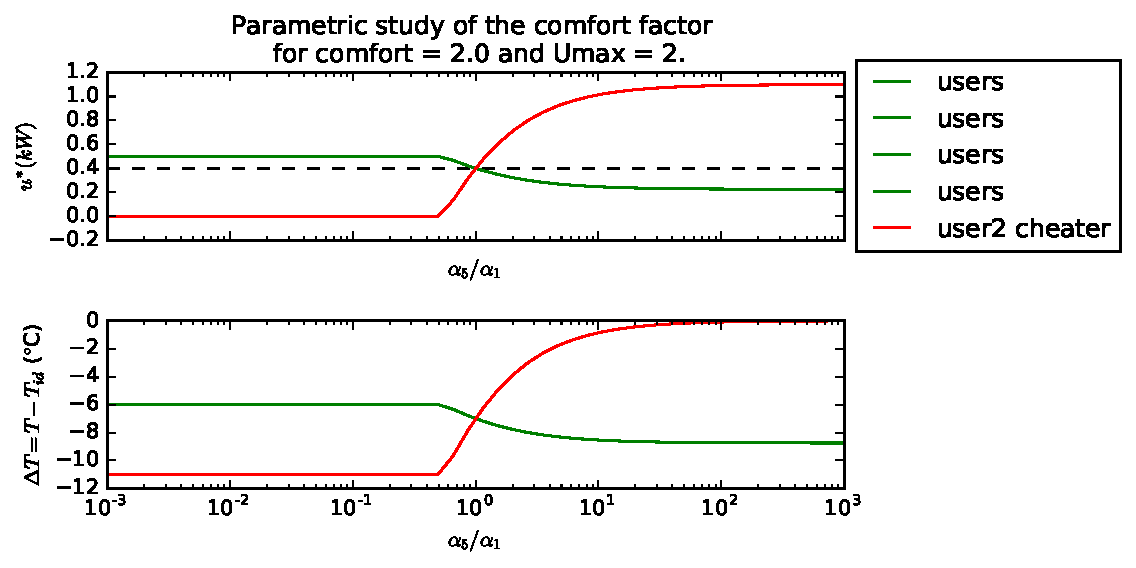
\includegraphics[width=3.5in]{statcht5alp.pdf}
\caption{Parametric study of the comfort factor for five users}
\label{SCHT_a5}
\end{figure}

Then, we wanted to determine the influence of the broadcasted ideal temperature on the distribution. In Figure \ref{SCHT_T} is represented the power distribution and the temperature deviation as functions of the broadcasted temperature. We notice that the higher this temperature is, the more energy the user receives and the less its deviation is. Please note that in our model if a user receives energy, this user has to consume it (hence the positive deviation in Figure \ref{SCHT_T}).
\begin{figure}[H]
\centering
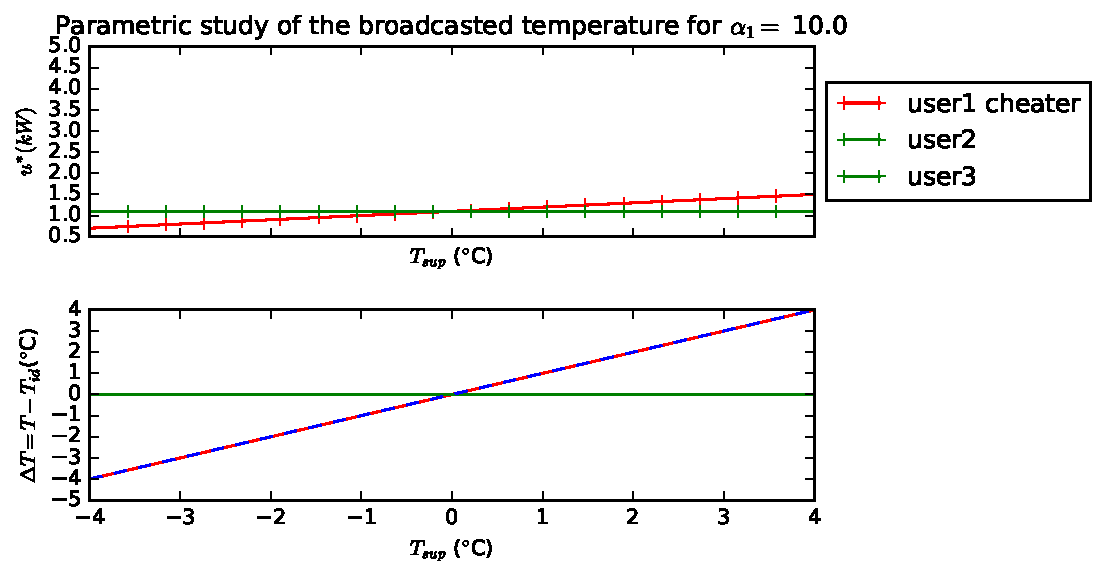
\includegraphics[width=3.5in]{statchtbcT.pdf}
\caption{Parametric study of the broadcasted ideal temperature when different from the real ideal temperature for three users}
\label{SCHT_T}
\end{figure}

%\begin{figure}[H]
%\centering
%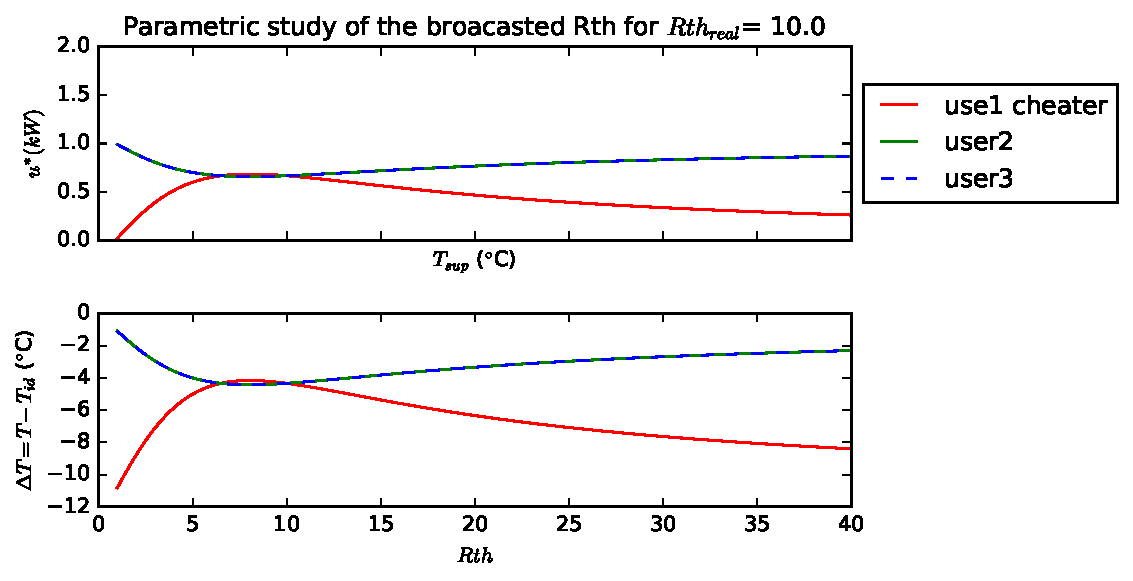
\includegraphics[width=3.5in]{statchtbcRth.pdf}
%\caption{Parametric study of the broadcasted thermal resistance when different from the real $R_{th}$ for three users}
%\label{SCHT_rth}
%\end{figure}

Finally, we created a situation where a user could listen or not to the talks of the DMPC. This means the user can decide if it takes into account the Lagrangian multiplier returned by the coordinator. We introduced this notion as the deafness $\beta$. If the user behaves and listen, $\beta = 0$, but if he is deaf,  and does not take the talk into account,  $\beta =1$. In Figure \ref{SRecal_i}, the nominal situation is presented and in Figure \ref{SRecal_} a situation were user 1 is deaf is presented. We do notice that when the user is deaf, its comfort is much better than when it listens to the talk. 
\begin{figure}[H]
\centering
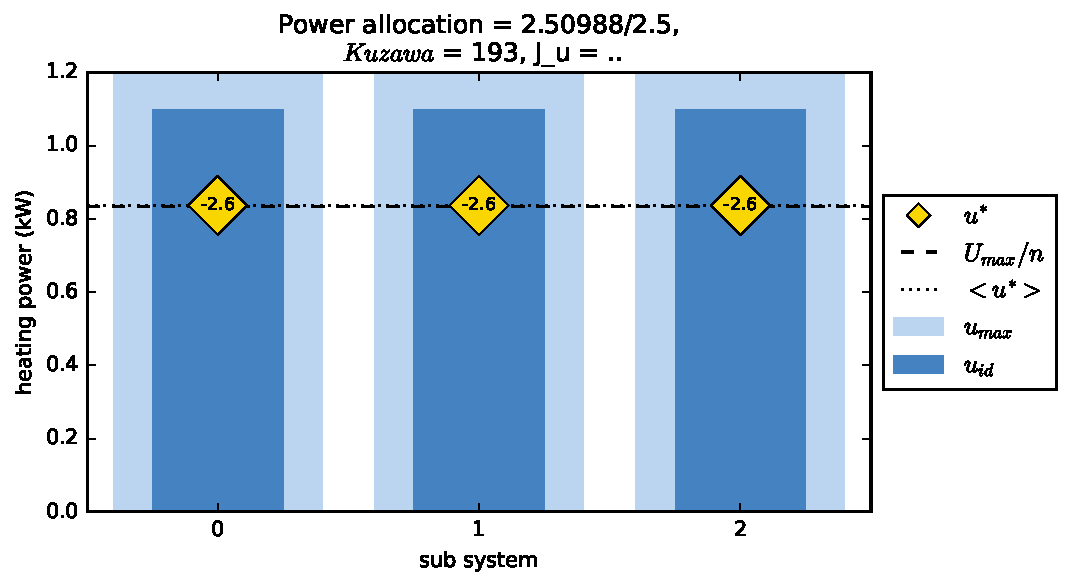
\includegraphics[width=3in]{StatRecal_init.pdf}
\caption{Power distribution for three user in the nominal case}
\label{SRecal_i}
\end{figure}

\begin{figure}[H]
\centering
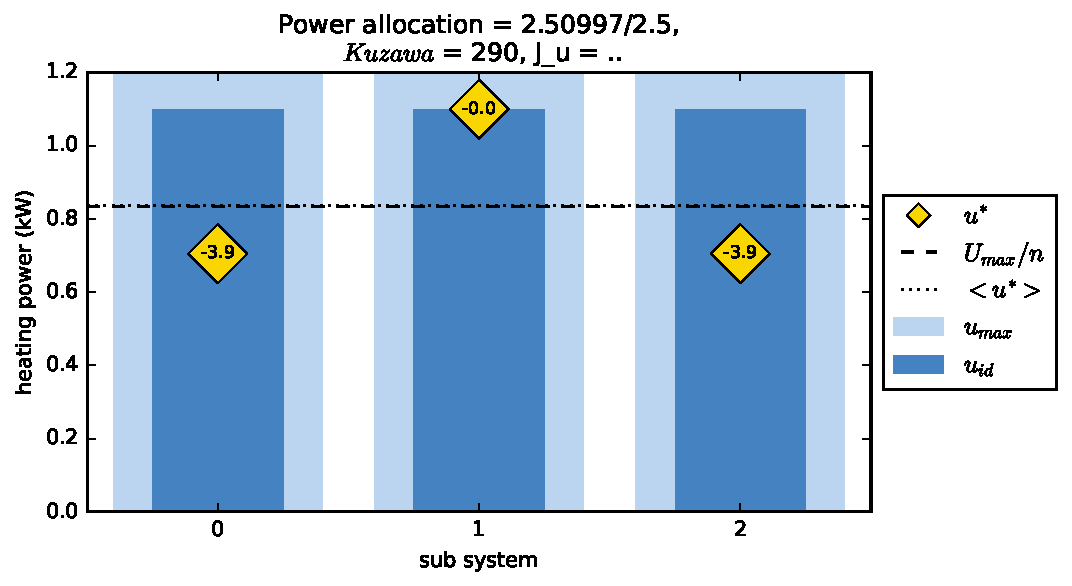
\includegraphics[width=3in]{StatRecal.pdf}
\caption{Power distribution for three users when user 1 does not listen to the talk}
\label{SRecal_}
\end{figure}
Of course this deafness factor $\beta$ can be set between 0 and 1. Figure \ref{SRecal_mult} shows the influence of the deafness factor of user 1 on the temperature deviation of both users. With no surprise, when a user is not listening to the talks all the others are depreciated.
\begin{figure}[H]
\centering
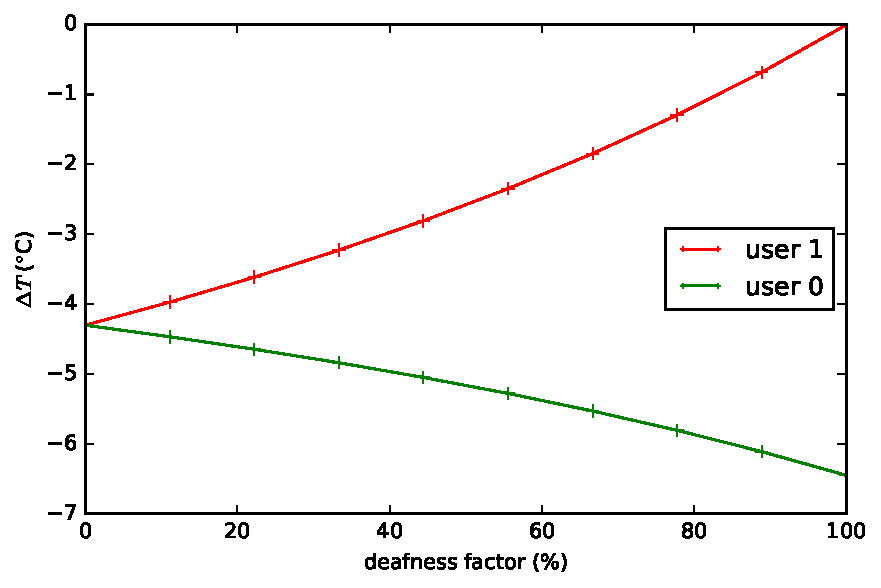
\includegraphics[width=3in]{param_mult.pdf}
\caption{Parametric study of the deafness factor on the deviation to ideal temperature}
\label{SRecal_mult}
\end{figure}

All those studies have been executed on the static model, but all those results can easily be extended to the dynamic model and to the DMPC. 

\subsection{Security in dynamic situations}
Now, let us consider the dynamic model. Our developed python module is able to deal with centralized MPC and distributed MPC. However, due to the complexity of the DMPC, its calculation requires more computation power. So for the sake of the simplicity the results of this part were obtained with a classic MPC but they can all be extended to the DMPC.  

\subsubsection{First, we consider a cheating user}
We want to observe the influence of the comfort factor. In Figures \ref{DMPCa_1} and \ref{DMPCa_2} we can observe the situation with two users. In blue we can see the the distribution in the nominal case were $\alpha_1=\alpha_2 = 10$. Then we change the value of the comfort factor for the second user. We notice that its comfort is drastically better (follows the reference temperature more than the green and the blue lines) to the detriment of the first user (in green).  

\begin{figure}[H]
\centering
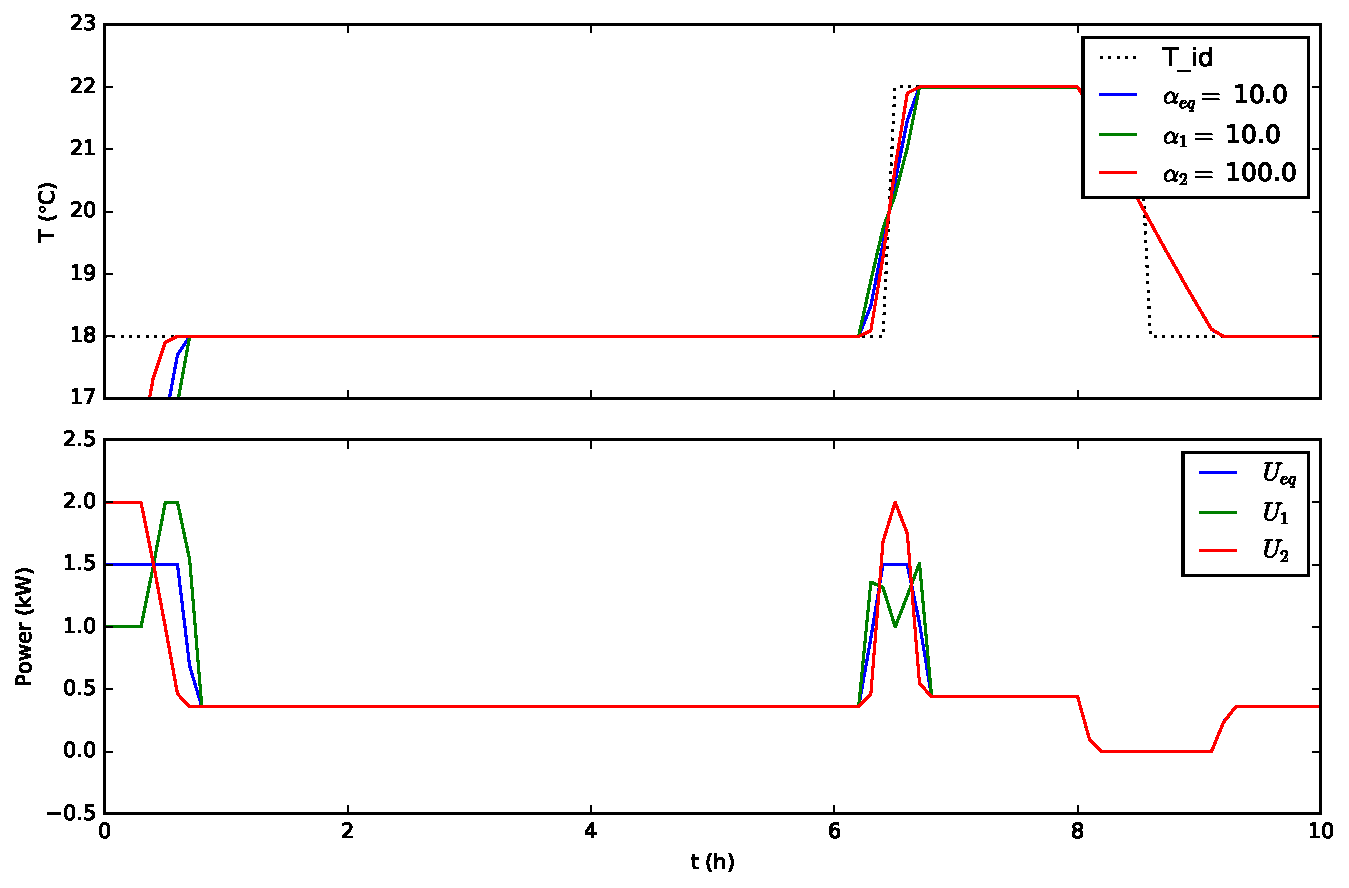
\includegraphics[width=3in]{DMPCalp.pdf}
\caption{Power distribution through time for two users. In blue is the nominal situation with identical comfort factor.}
\label{DMPCa_1}
\end{figure}

\begin{figure}[H]
\centering
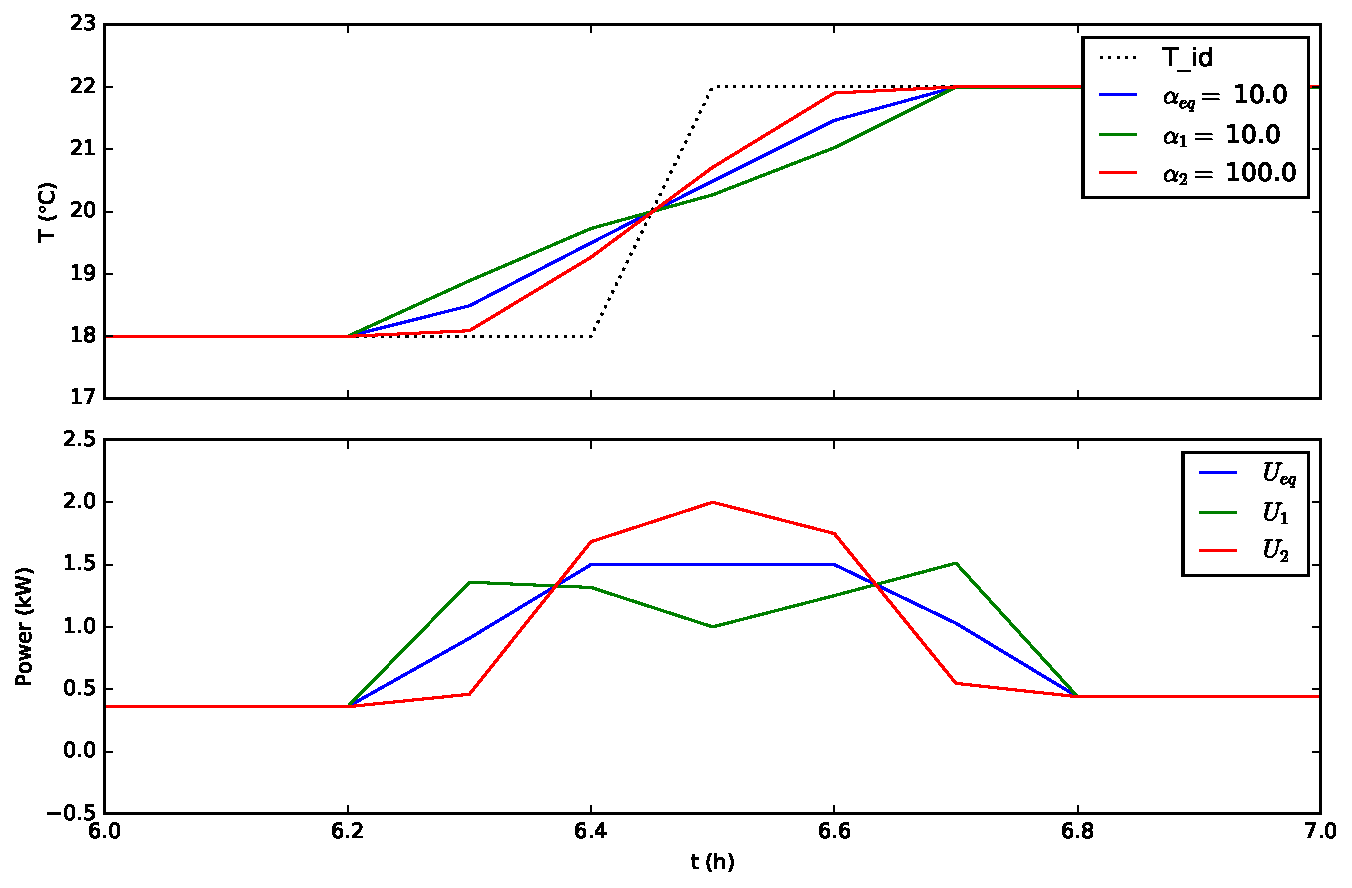
\includegraphics[width=3in]{DMPCalpZ.pdf}
\caption{Power distribution through time for two users. In blue is the nominal situation with identical comfort factor. Focus between 6\hc 00-7\hc 00 am}
\label{DMPCa_2}
\end{figure}

Our study pointed out that the more $\alpha_2 > \alpha_1$, the more user 2 has a great comfort and the opposite for user 1. Hence, by modifying $\alpha$, one could easily cheat the DMPC in order to gain access to more energy.


\subsubsection{Then, we consider a nihilist user.}
As previously stated, a nihilist user is a user whose objective is to disrupt the system and even destroy it. In our first subsection, we presented several strategies in order to disable the DMPC system.  During this phase, we evaluated the influence of different parameters to detect if they could be a liability in the DMPC. We notice that by augmenting the comfort factor of all users, we could reach a threshold and make the Uzawa iteration not converging (or at least reaching the maximum admissible iteration $k_{max}$). Hence if a user succeeds to change the value of all the $\alpha$, it might be able to break the DMPC. 

Secondly, we tried the other method : to use a particular sequence of $u^*_i[k]$ and not the result of the optimization. We created a sequence such as $u_2[k] = u^i_{max}$ if k is an odd number and  $u_2[k]=0$ else.  In Figure \ref{Nihil_1}, we show the distribution through time for the non-nihilist user (user 1). In Figure \ref{Nihil_2}, we show the same but for the nihilist user (user 2).
\begin{figure}[H]
\centering
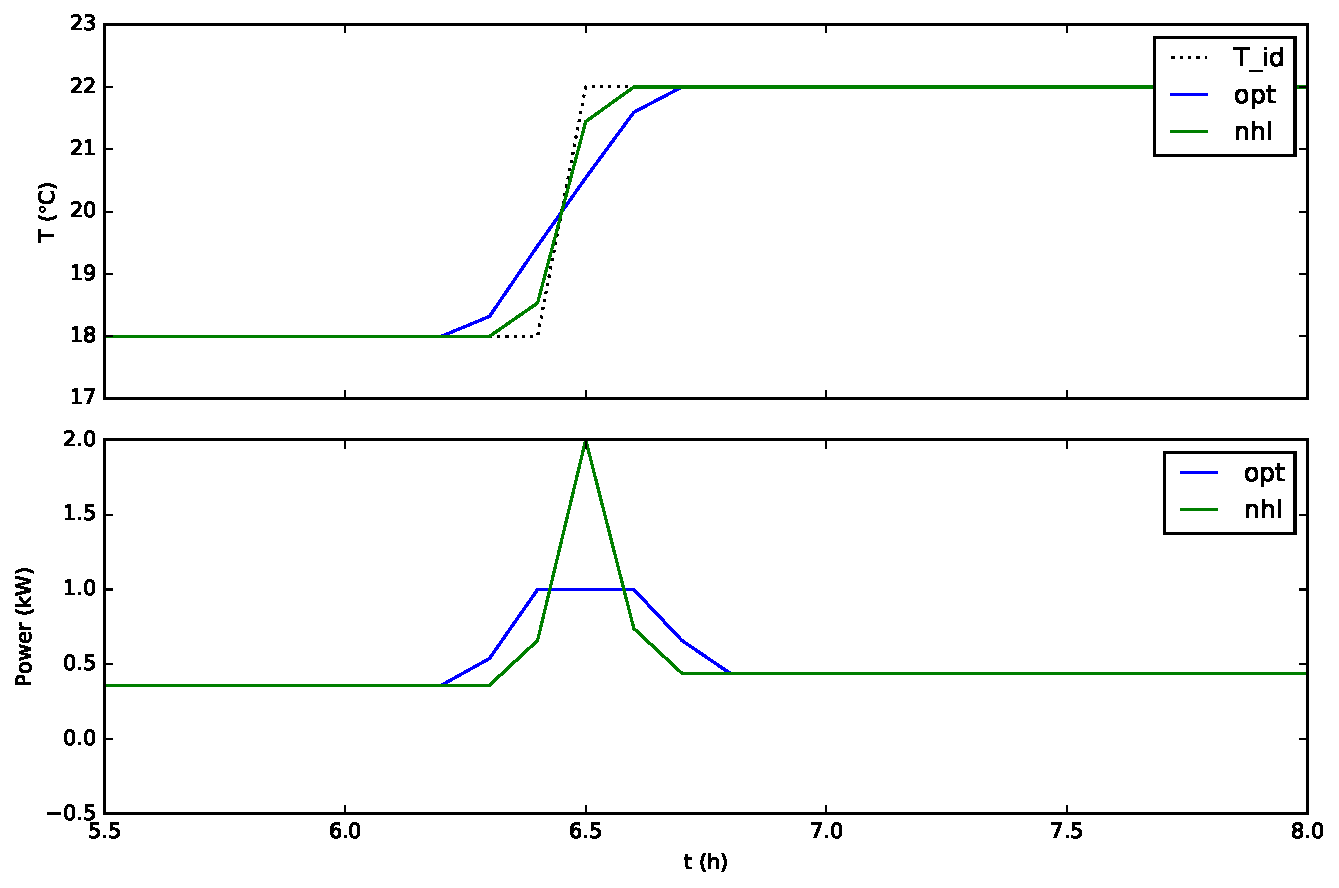
\includegraphics[width=3in]{NihilSeq_init.pdf}
\caption{Power distribution through time for user 1 when applying a destroying sequence of consumed power for user 1}
\label{Nihil_1}
\end{figure}

\begin{figure}[H]
\centering
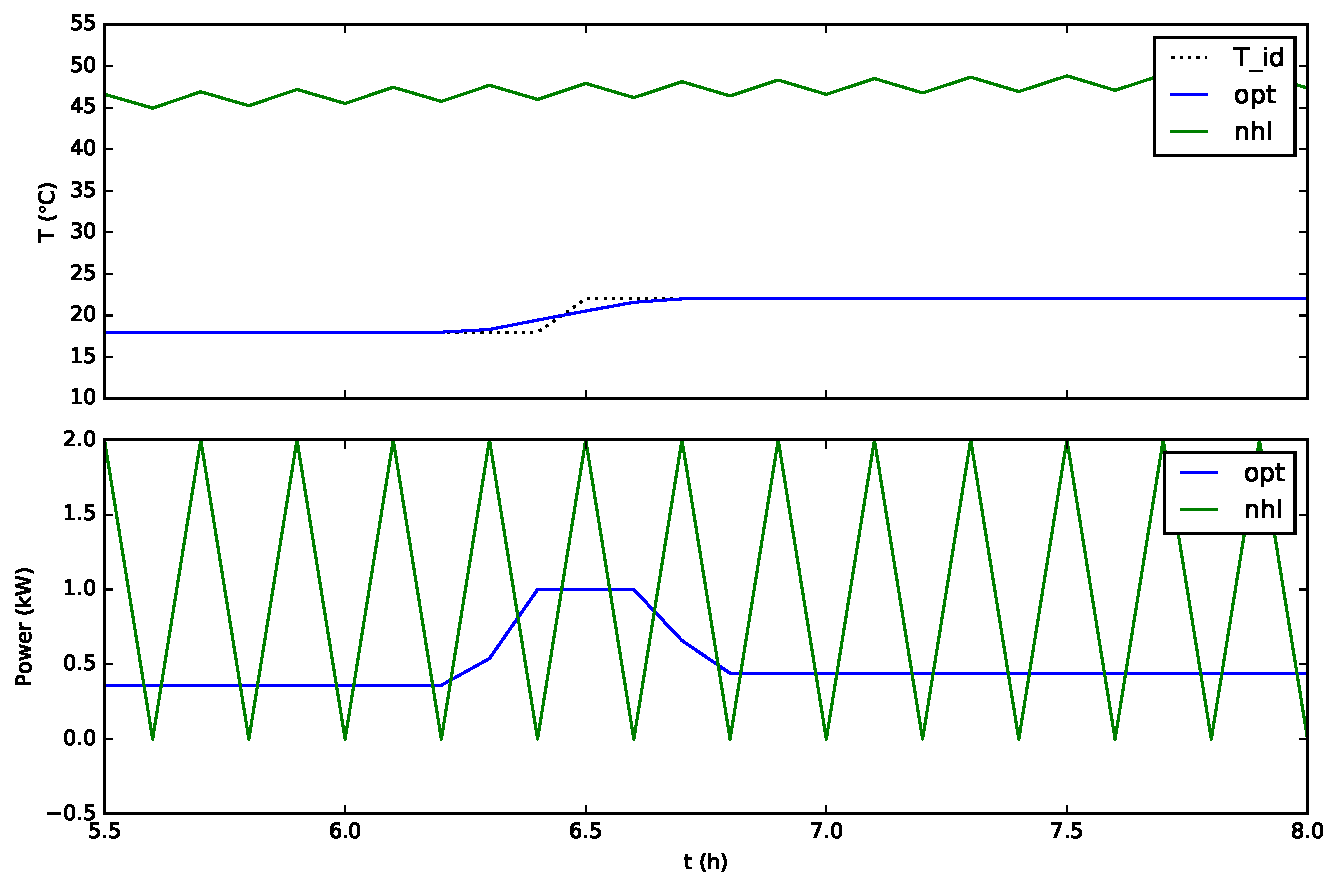
\includegraphics[width=3in]{NihilSeq.pdf}
\caption{Power distribution through time for user 0 when applying a destroying sequence of consumed power for user 1}
\label{Nihil_2}
\end{figure}

When summing $u^*_1$ and $u^*_2$ we notice that the max is superior to the amount of energy available $U_{max}$. This proves that this sequence disable the DMPC. 

\subsection{Protection}
Finally, we studied security counter-measures against those threat. We noticed through our experiment that when we were altering the parameters, we modified as well the following functions :
\begin{itemize}
\item[•] $k_{Uzawa} \rightarrow (u^*(k_{Uzawa}) | \alpha)$
\item[•] $\lambda \rightarrow (u^*(\lambda) | \alpha)$
\item[•] $k_{Uzawa} \rightarrow (\lambda (k_{Uzawa}) | \alpha)$
\end{itemize} 
In other words, the first (\textit{resp.} second) function represents the power distribution (of one user for a given $\alpha$) as a function of the number of iteration realized in the Uzawa method (\textit{resp.} the value of the Lagrangian multiplier). Similarly, the third one returns the value of the Lagrangian multiplier as a function of the number of iteration realized in the Uzawa method. 

In Figure \ref{CM_1}, we can observe the nominal situation. Then in Figure \ref{CM_2} we can see a cluster of lines created for different values of $\alpha$.

\begin{figure}[!t]
\centering
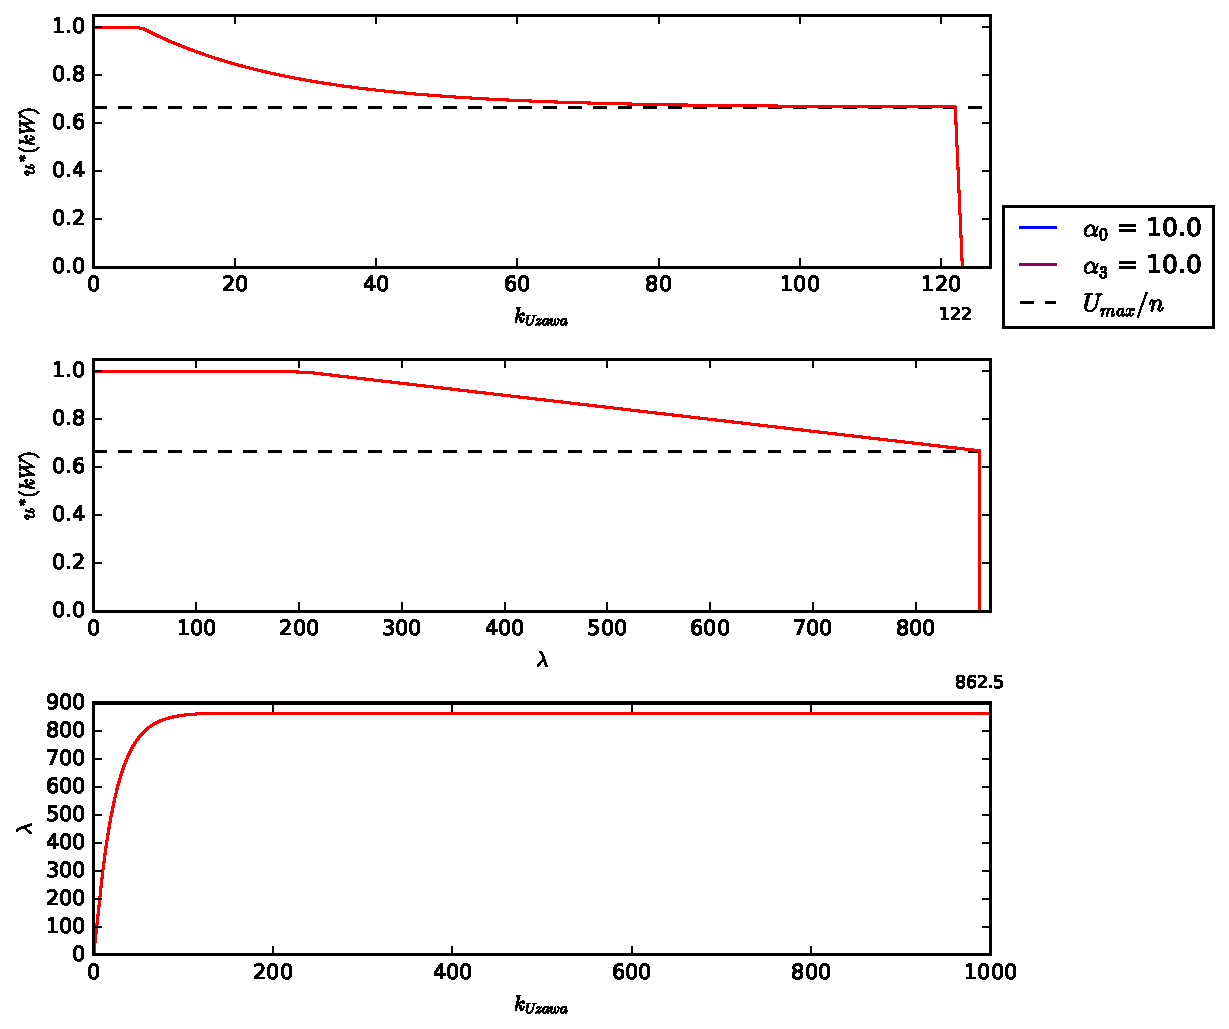
\includegraphics[width=3in]{KL_init.pdf}
\caption{$u^*(k)$, $u^*(\lambda)$ and $\lambda(k)$ in nominal situation}
\label{CM_1}
\end{figure}

\begin{figure}[!t]
\centering
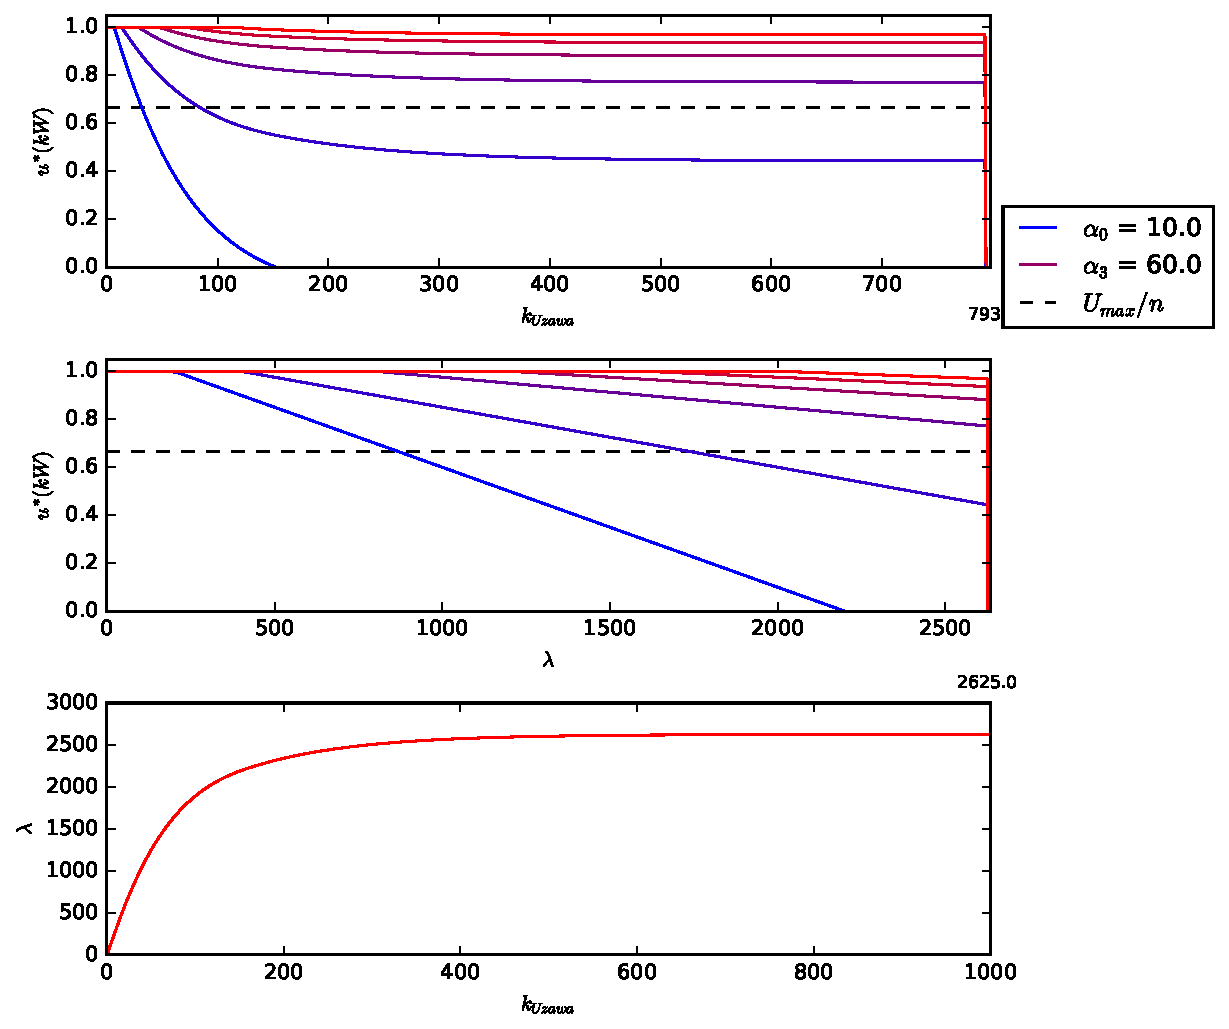
\includegraphics[width=3in]{KL_10-80.pdf}
\caption{Parametric study of the influence of the comfort on different functions. Comfort factor $\alpha_i \in {10, 20, 40, 60, 80, 100}$.}
\label{CM_2}
\end{figure}

We then decided to realize a large cluster of lines for alpha linearly distributed. The result is presented in Figure \ref{CM_3} for $\alpha$ in range 0 to 150. 

\begin{figure}[!t]
\centering
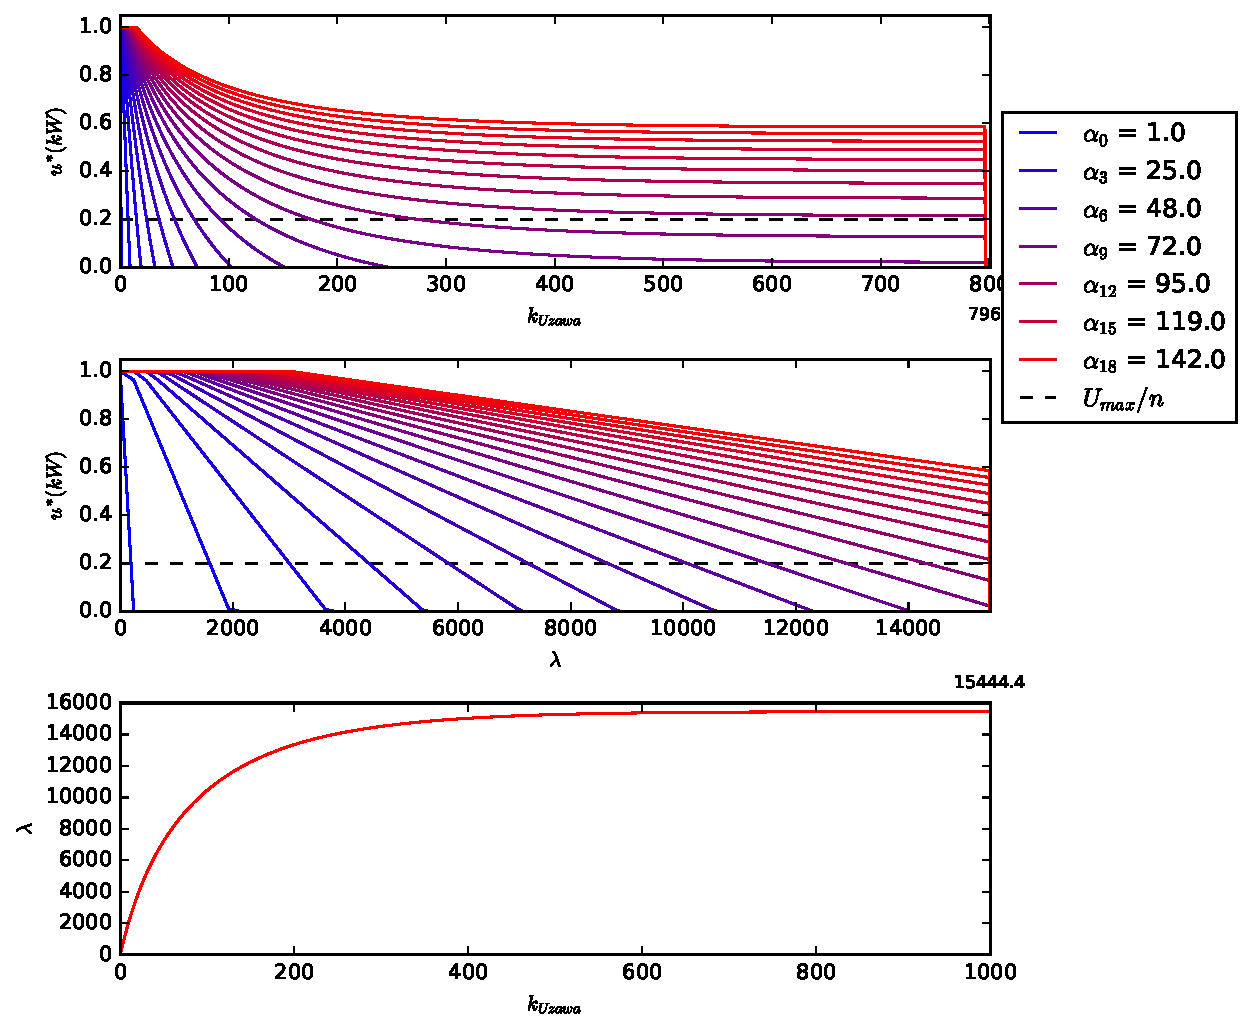
\includegraphics[width=3in]{KL_lin.pdf}
\caption{Parametric study of the influence of the comfort on different functions. Linear distribution of comfort factor.}
\label{CM_3}
\end{figure}

Thanks to Figure \ref{CM_3}, we can set a threshold (for instance on the line $\alpha_{12}$), this will divide the space in two : above the line $(u^*(k_{Uzawa}) | \alpha_{12})$, user will be considered as cheaters, else the users are cleared. Respectively below the line $(u^*(\lambda) | \alpha_{12})$, user will be considered as cheaters, else the users are cleared.

This is a way to detect efficiently cheating and nihilist users using a comfort variation approach.  


\section{Conclusion}
In this paper, we presented new results on security breach and measures for distributed model predictive control. By developing a thermal model we were able to experiment various approaches on,  firstly,  how to destroy or cheat, and secondly on how to detect such behaviours. By analysing all  the different method, we managed to reduce those situation to a few base cases much easier to analyse and export to other situations. All those results are encouraging and call for further investigation on the subject. 

\bibliographystyle{ieeetr}
\bibliography{biblio_BSCa}

\end{document}


